% This is samplepaper.tex, a sample chapter demonstrating the
% LLNCS macro package for Springer Computer Science proceedings;
% Version 2.20 of 2017/10/04
%
\documentclass[runningheads]{llncs}
%
\usepackage{graphicx}
% Used for displaying a sample figure. If possible, figure files should
% be included in EPS format.
%
% If you use the hyperref package, please uncomment the following line
% to display URLs in blue roman font according to Springer's eBook style:
% \renewcommand\UrlFont{\color{blue}\rmfamily}

\begin{document}
%
\title{Admission Handler}

\author{Group 18: Jan Haas \and Simon Hauser \and Sam Kenworthy}

\institute{}
%
\maketitle              % typeset the header of the contribution

\section{Introduction}
This project implements a distributed admission system for large events and venues with limited capacity.
The stream of visitors entering or exiting the venue will be monitored in real-time via mobile devices at each entrance.
Live feedback will be provided to each device, enabling organizers to stop admission when the maximum capacity of the venue has been reached.

As the world starts to reopen after the pandemic and public events become possible again, systems are required to handle the keeping of safe capacities, in-line with changing guidelines and laws.
Pre-selling tickets is one possibility of managing these limits, yet events such as Christmas markets, beer gardens and public concerts live off spontaneous visits.
This project will enable the simple monitoring and managing of such streams of visitors, by providing a dynamically scalable system by using end-user mobile devices as client-hosts.
\section{Requirements Analysis}
New mobile clients join the system by broadcasting a request and establishing a TCP connection with the first server to answer them.
They communicate newly arriving guest to this server and only allow passage if they get a positive response.
Each server response, as well as periodic polls in case a client does not have new guests arriving for a time pass the client the current number of guests still allowed inside for display.
If a client does not receive an answer from its associated server, it tries to find a new one via the same process as a freshly joining one. If a server does not hear from a client, the TCP connection is simply purged.

A fresh server joins the system by broadcasting a join request.
If it does not receive answers, it establishes itself as the new system with zero current guests.
If it does get an answer, the number of arrivals is synchronized between servers.
To ensure a fair entry process and for possible other uses, arrivals are causally ordered.
New arrivals are only passed if they have been integrated in the causal order and are not over capacity according to it.

We are still debating if servers elect a leader or establish a peer-to-peer connection and only vote on the correctness of the causal order of entries.
While a leader would help in case of ties occurring while voting on the correct order of arrivals, it also makes the other servers seem hardly useful.

If a server loses an established connection to a system, it notifies connected clients and goes dormant until it is able to reestablish the connection.
This ensures that the venue does not go over capacity from having two independent systems exist.
From the system side, if a single server cannot be reached anymore, other servers simply close the connection to it.
If a problem occurs that separates the system into two parts of 2+ servers ... %TODO
If the possible leader loses connection, the other servers elect a new one.
To ensure that a recovery process can be started early, either the leader or each peer sends periodic life signs and starts the recovery process if there is no answer (from one of the servers).
\section{Architecture}
%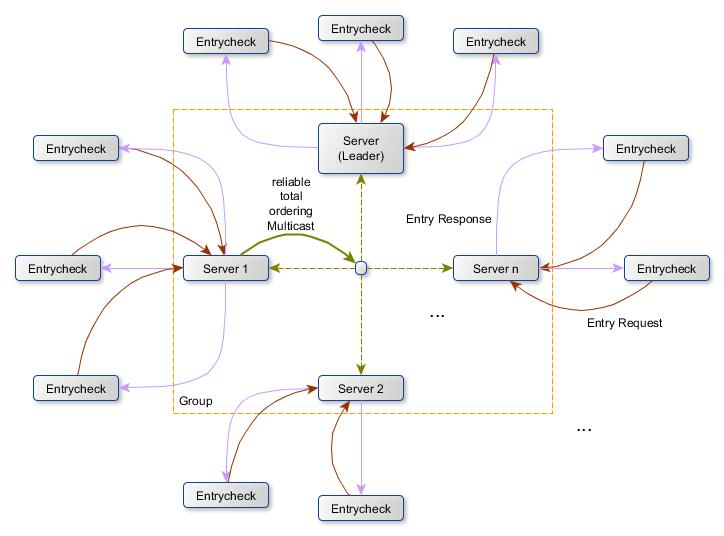
\includegraphics[width=\textwidth]{architecture_graph.jpg}

\end{document}
